%!TEX root = ../../../super_main.tex

\chapter{Screenshots of the Finished Applications and Components}
Throughout the following sections screenshots of the shared components will be shown while showcasing the developed applications.
\todo[inline]{plox read - no author ever )aka feupeu( )}

\section{\launcher.}
The following screenshots are from the \launcher application.

\begin{figure}[!htbp]
	\centering
	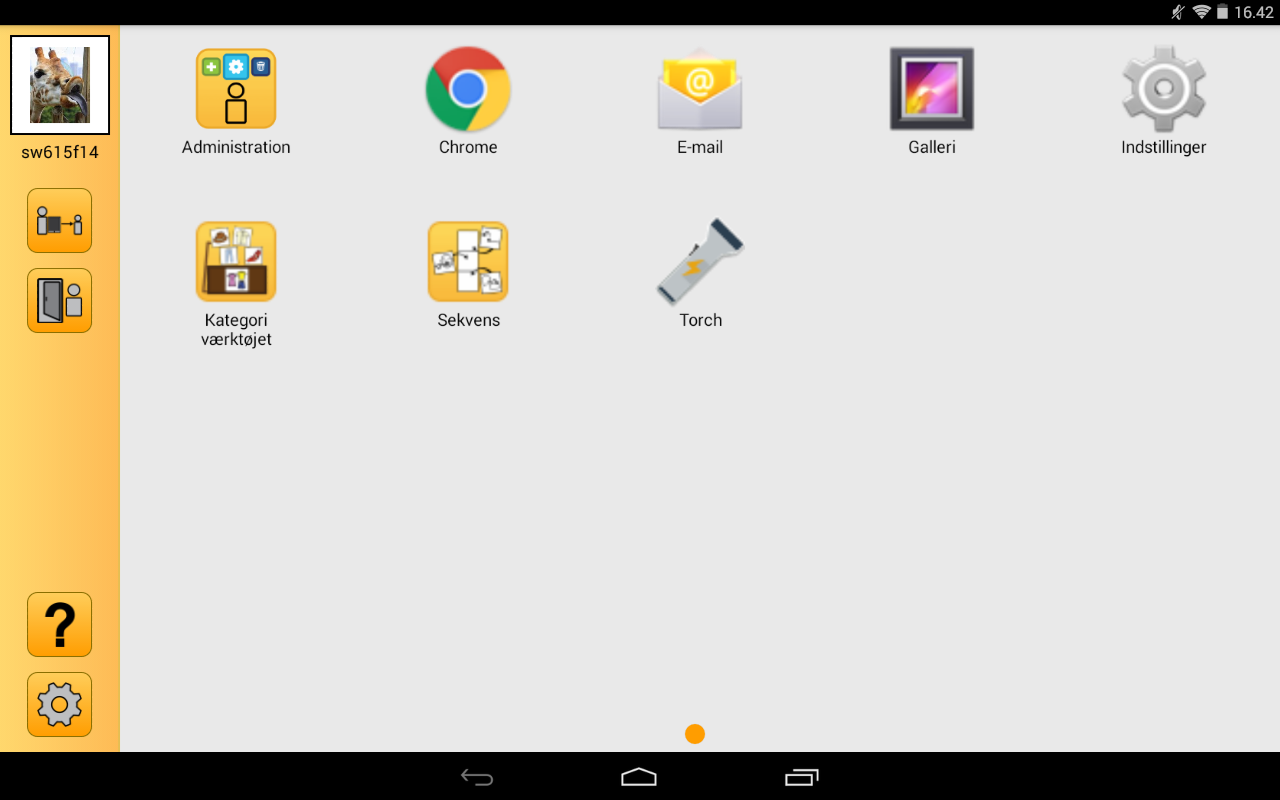
\includegraphics[width=\textwidth]{finished/3}
	\caption{The grid of applications on the home screen of the \launcher}
\end{figure}
\FloatBarrier

\begin{figure}[!htbp]
	\centering
	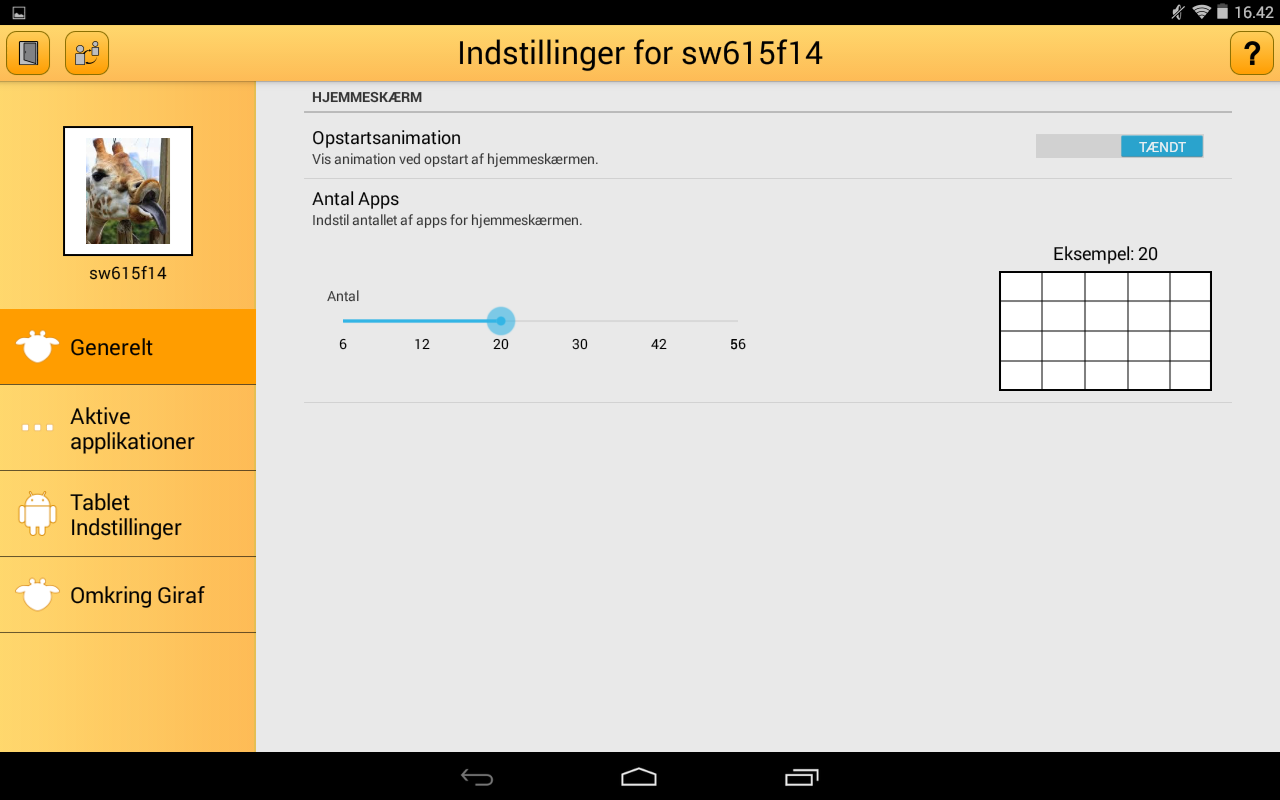
\includegraphics[width=\textwidth]{finished/4}
	\caption{The settings panel of the \launcher}
\end{figure}
\FloatBarrier

\begin{figure}[!htbp]
	\centering
	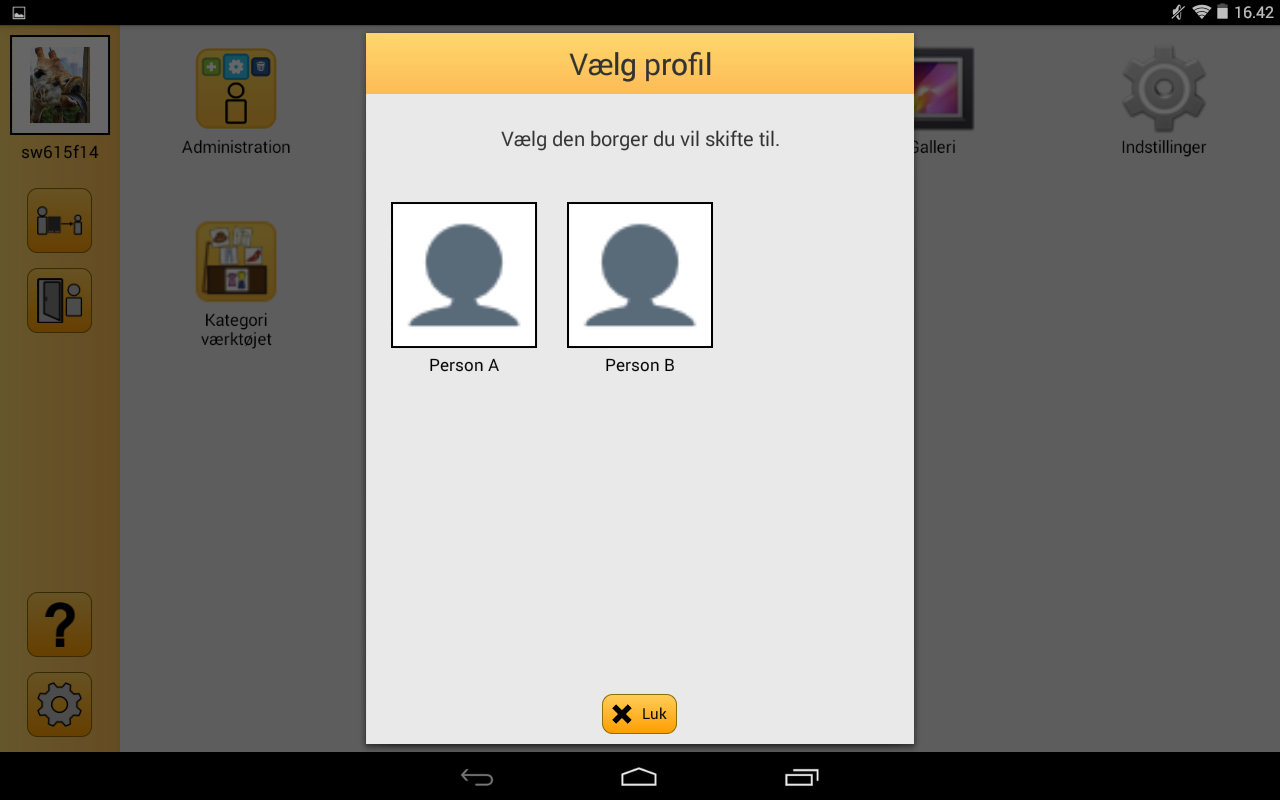
\includegraphics[width=\textwidth]{finished/5}
	\caption{One of the developed dialogs used to change profile}
\end{figure}
\FloatBarrier

\begin{figure}[!htbp]
	\centering
	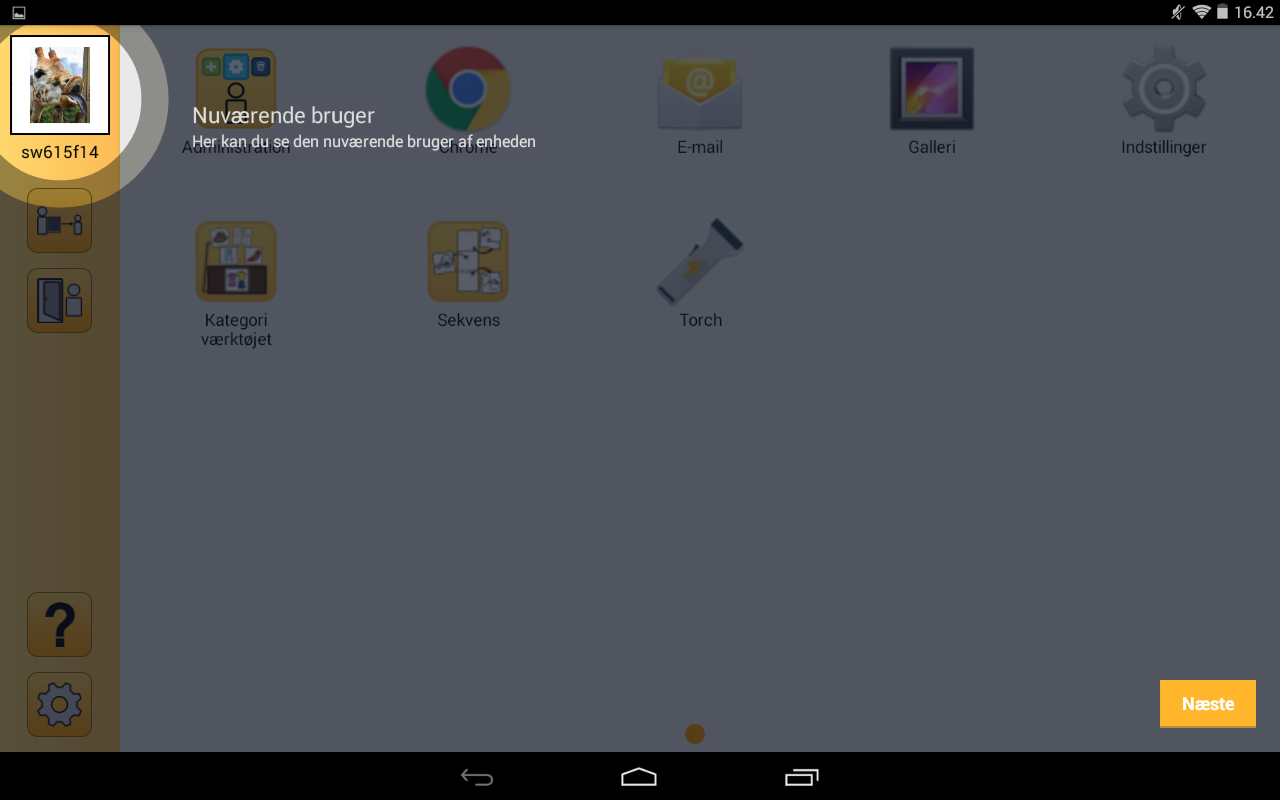
\includegraphics[width=\textwidth]{finished/6}
	\caption{An example of the helpful guide implemented}
\end{figure}
\FloatBarrier

\begin{figure}[!htbp]
	\centering
	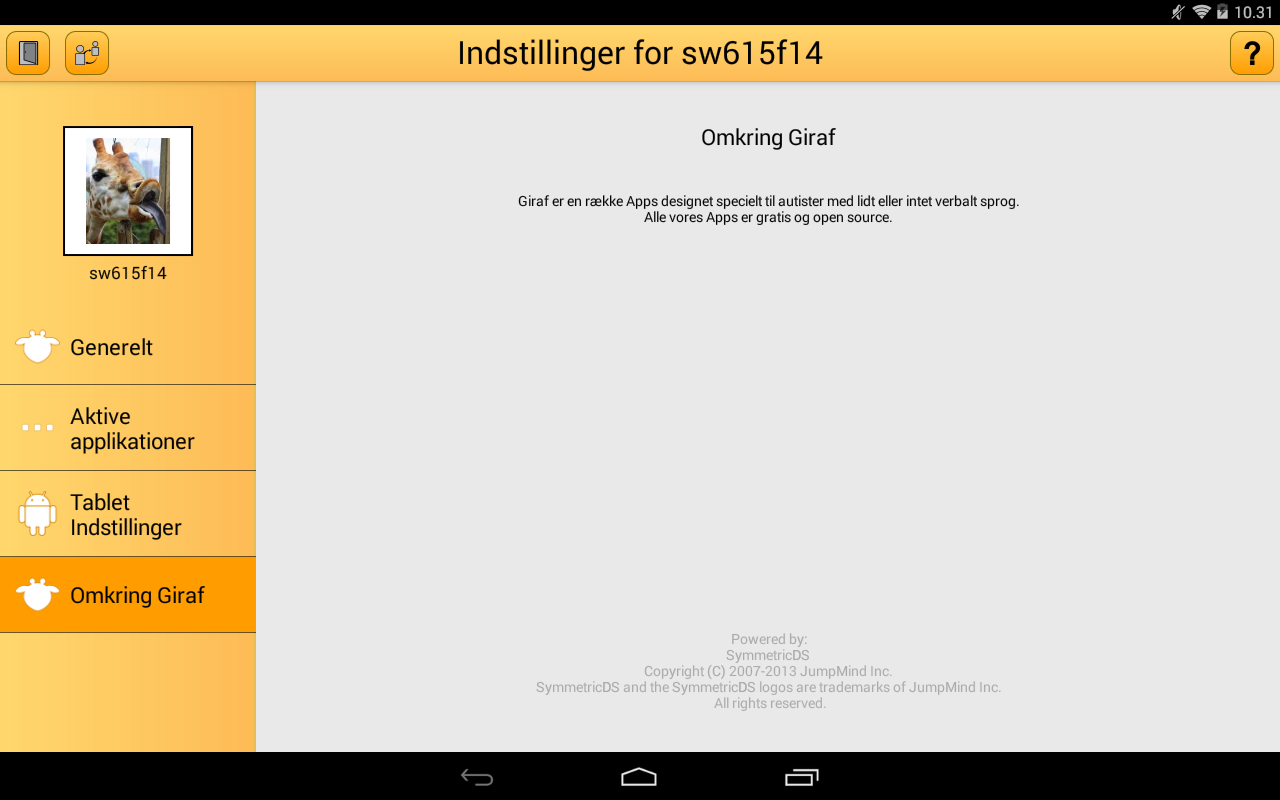
\includegraphics[width=\textwidth]{finished/1}
	\caption{The about giraf page}
\end{figure}
\FloatBarrier

\begin{figure}[!htbp]
	\centering
	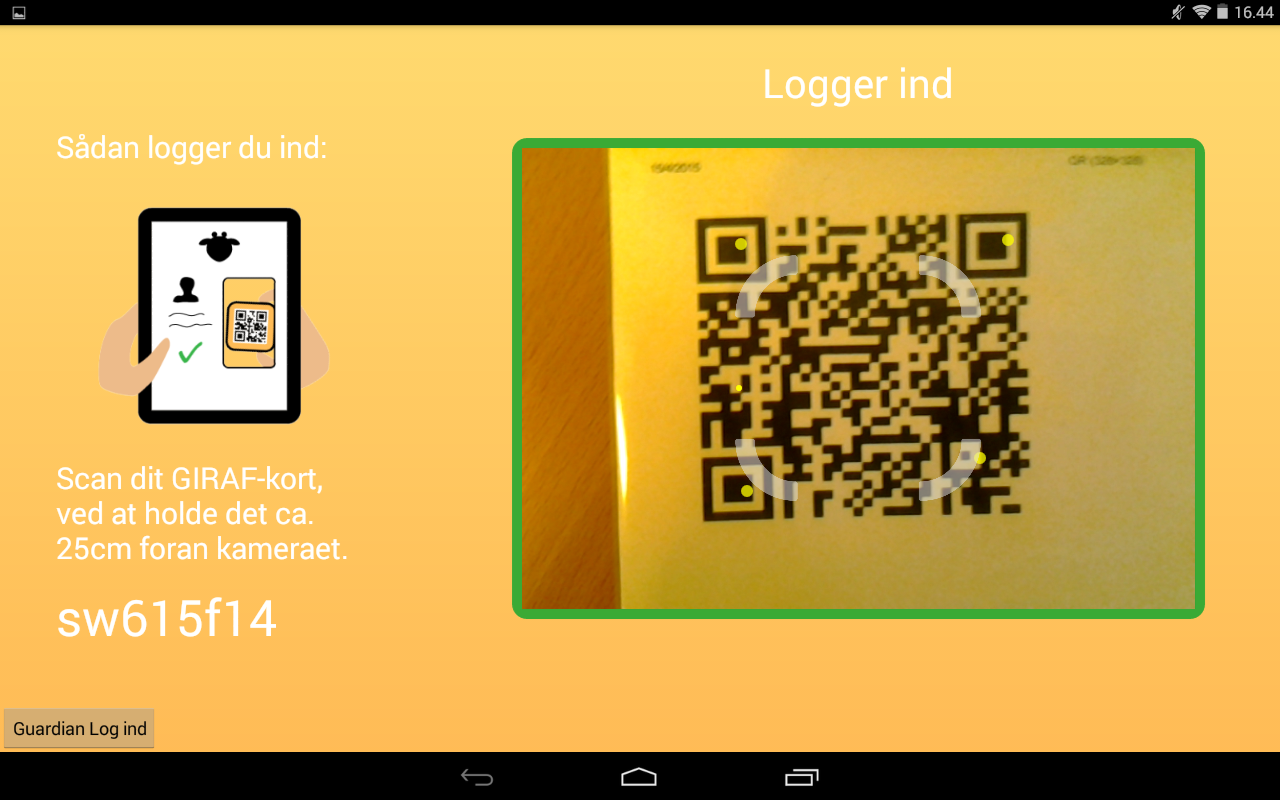
\includegraphics[width=\textwidth]{finished/7}
	\caption{The login / authentication screen}
\end{figure}
\FloatBarrier

\section{\ct}
The following screenshots are from the \ct application.

\begin{figure}[!htbp]
	\centering
	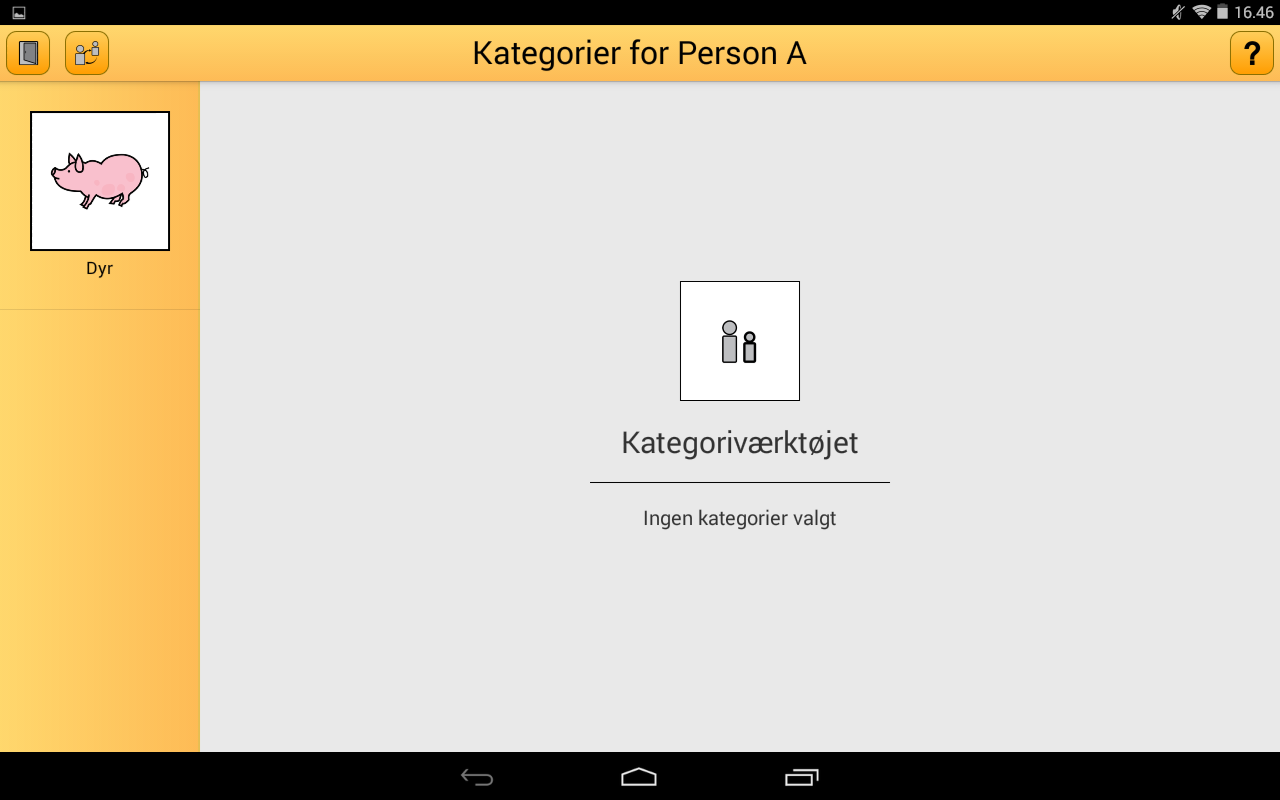
\includegraphics[width=\textwidth]{finished/13}
	\caption{The initial screen of the \ct}
\end{figure}
\FloatBarrier

\begin{figure}[!htbp]
	\centering
	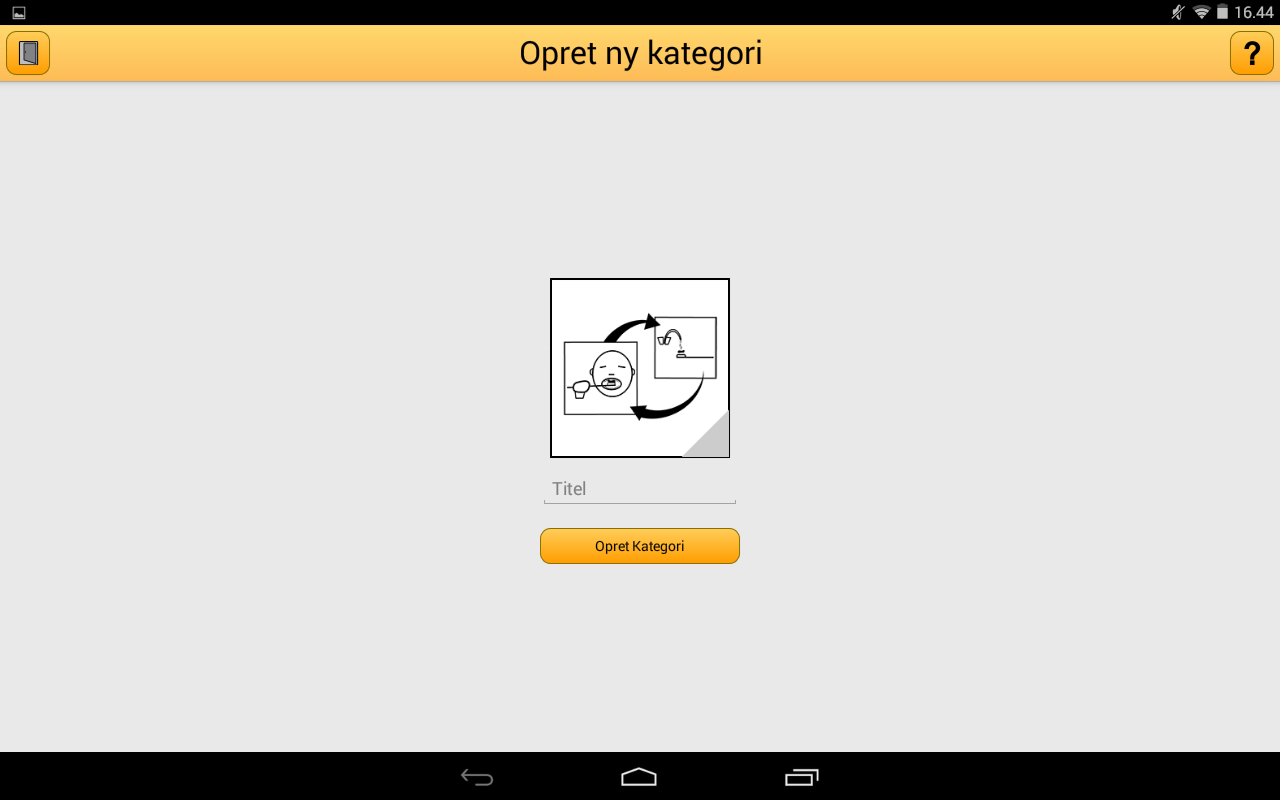
\includegraphics[width=\textwidth]{finished/8}
	\caption{The create category screen}
\end{figure}
\FloatBarrier

\begin{figure}[!htbp]
	\centering
	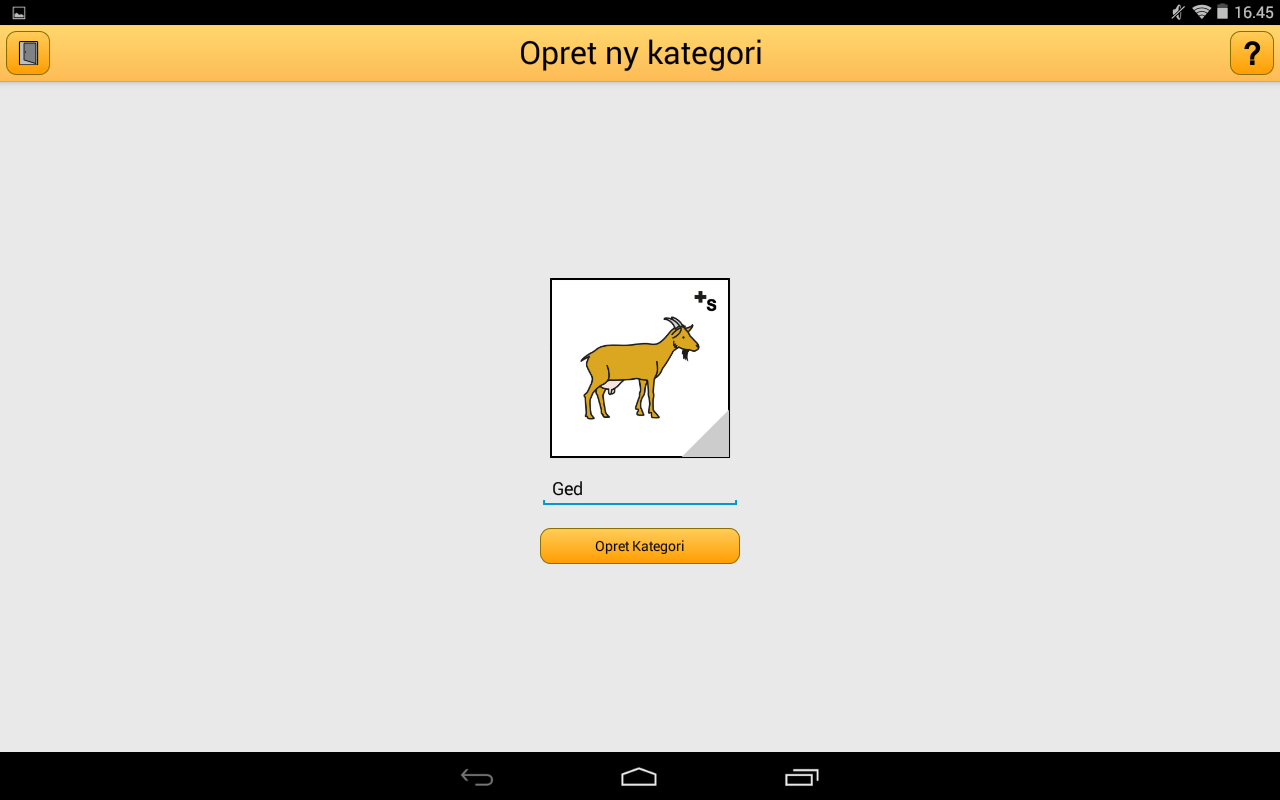
\includegraphics[width=\textwidth]{finished/9}
	\caption{The create category screen with data}
\end{figure}
\FloatBarrier

\begin{figure}[!htbp]
	\centering
	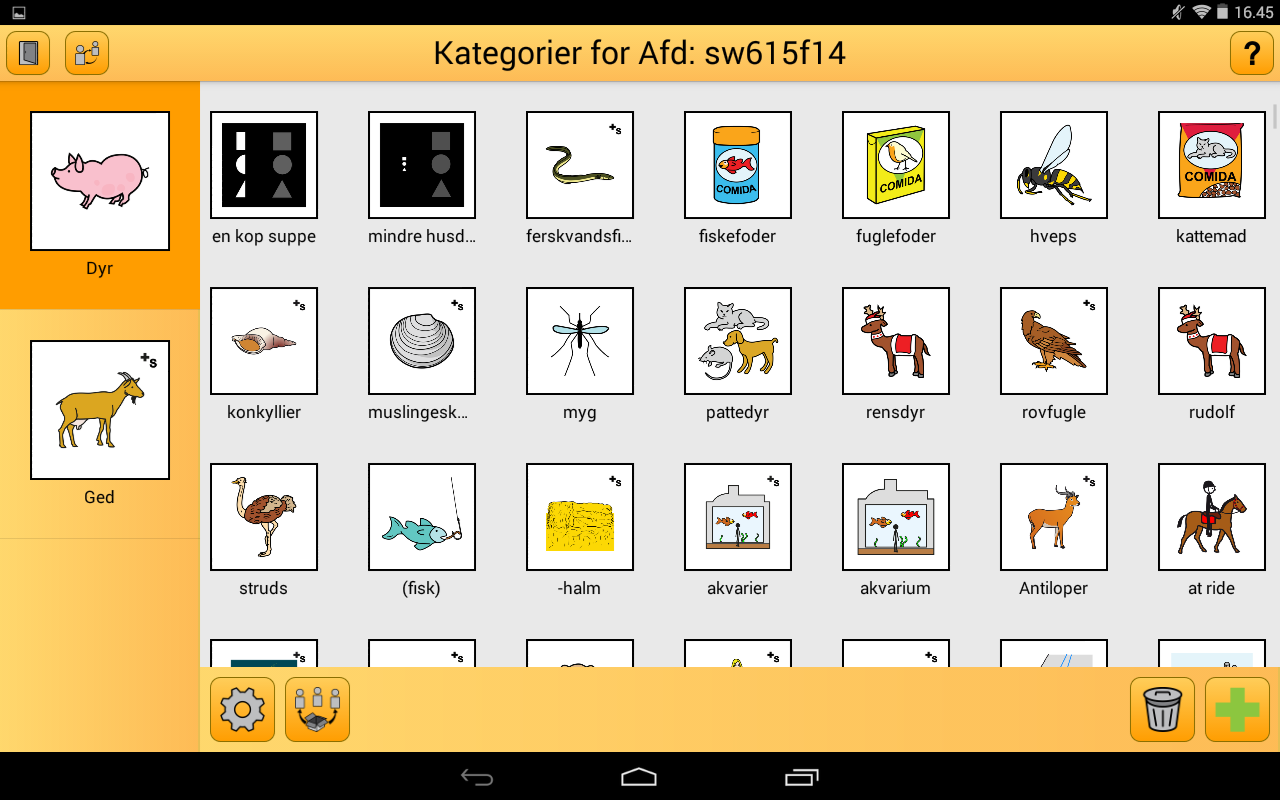
\includegraphics[width=\textwidth]{finished/10}
	\caption{The view where the category ``dyr'' selected}
\end{figure}
\FloatBarrier

\begin{figure}[!htbp]
	\centering
	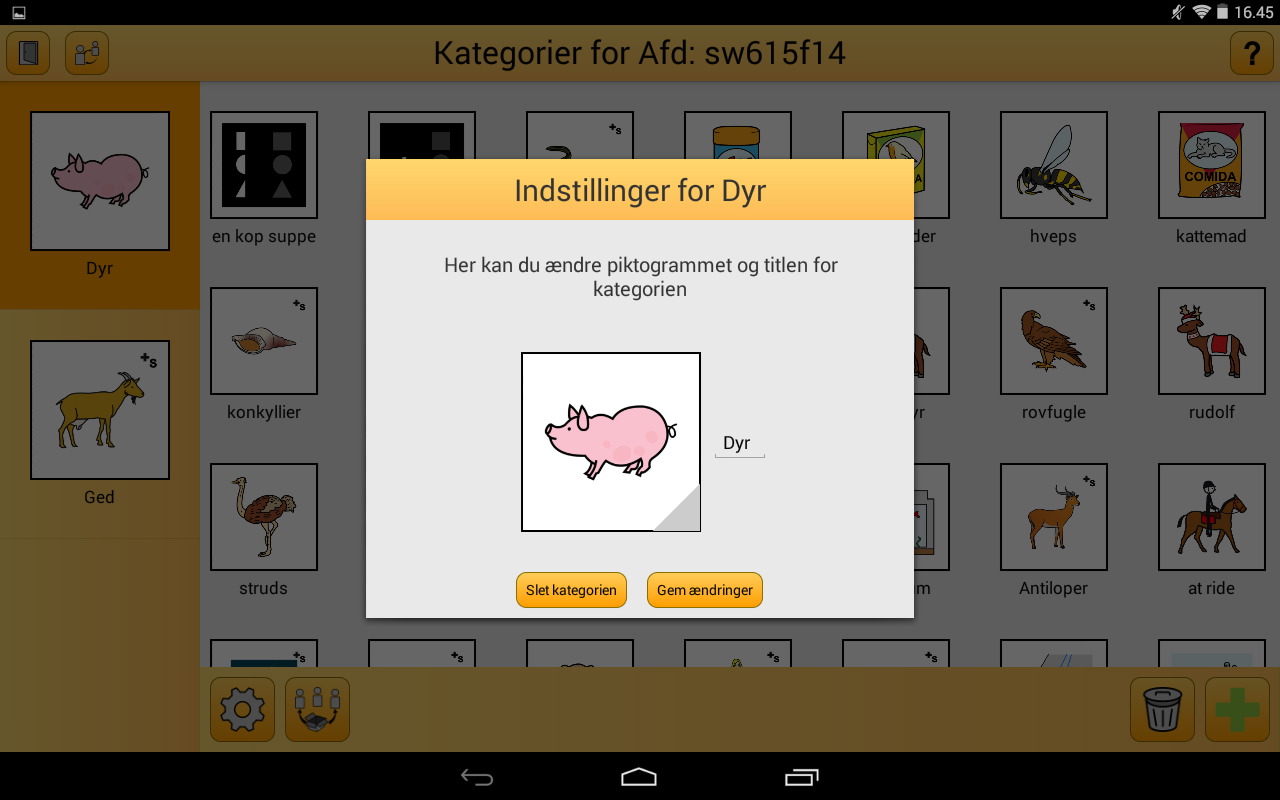
\includegraphics[width=\textwidth]{finished/11}
	\caption{The settings-dialog for the category ``dyr''}
\end{figure}
\FloatBarrier

\begin{figure}[!htbp]
	\centering
	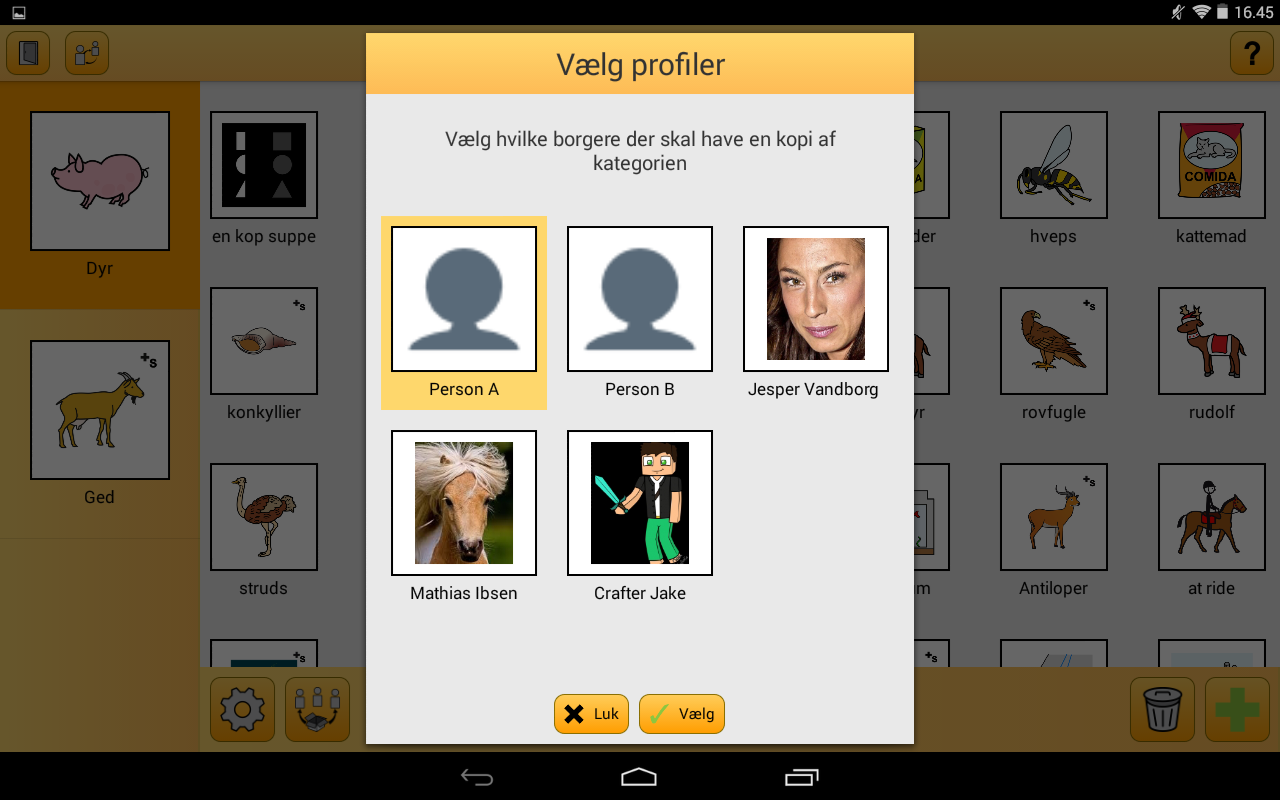
\includegraphics[width=\textwidth]{finished/12}
	\caption{The dialog used to assign categories to users}
\end{figure}
\FloatBarrier